\section{Agent-Coordinated Task-Level Operation}
\label{sec:closed-loop-operation}

A task supplies a process objective and the active production context, including line, product, and run. Fig.~\ref{fig:agent-loop} shows the conceptual task-to-write workflow in the current design, not a successful live-Agent run from this evaluation. The task context alone does not authorize a device write. The control node is resolved from an explicit \texttt{control\_node\_id} or the Agent's DCW/recipe binding. The data-acquisition (DAQ) target is resolved from an explicit target ID or the Agent's DAQ binding; a read-only node visible through the channel line is also eligible. Section~\ref{sec:eval} reports the scripted process results separately from the negative live-Agent pilot.

In goal-mode execution, a Lead Agent may decompose the objective, dispatch subtasks to worker agents, and judge completion. This optional coordination organizes the task but does not define a control policy. For each control step, the responsible Agent invokes \texttt{optimization\_explore}, which performs the checks before device I/O.

The operation resolves the optimization profile and control-node binding, then uses the node's stored value as the current setpoint $u_0$. This value is not necessarily a fresh device readback. If direction is omitted, the operation defaults to an upward adjustment; otherwise, the supplied direction determines $s\in\{-1,+1\}$. For a step $\Delta u$, it forms
\begin{equation}
 u^{*}=\operatorname{clip}\!\left(u_0+s\Delta u,\,u_{\min},\,u_{\max}\right),
 \label{eq:optimization-candidate}
\end{equation}
where configured tuning bounds take precedence; node bounds are used otherwise. The effective step is selected in this order: an explicit argument, the binding's tuning step, the scene's maximum step, or one twentieth of the node range.

The operation then resolves the DAQ target and verifies its visibility. In the later source implementation (commits \texttt{1aa4b136} and \texttt{66a8d5b5}), an optional identifiability preflight checks the control node's intervention ledger: an unclosed prior intervention or an unexpired recommended window after an underpowered or confounded verdict blocks a new step. A model--ontology cross-check treats missing evidence as unknown; a confirmed conflict rejects an automatic request; on the manual path, this cross-check does not itself block dispatch. Either gate can be disabled by configuration. If the checks pass, the operation attempts a pre-write DAQ read; its mean may be unavailable. These later checks are design features, not results attributed to the November 1 experiments, whose manifests name \texttt{da627d21} and whose active services were not captured as a hermetic snapshot.

A valid candidate enters the shared write-control path, which resolves the applicable binding and authority and determines whether the route requires approval. Only a gated route waits for approval. After approval, the path rechecks authorization and binding; the common controller applies the effective range and, for agent or manual writes outside benchmark mode, the applicable step, timing, and hold constraints before calling the configured driver. A route without an approval gate skips the wait but still passes through the common controller checks. A write denial or approval decline is recorded as rejected without driver dispatch. A driver-stage error may also be recorded as rejected after dispatch has begun, so status alone cannot establish whether the device changed; the caller must read and reconcile device state before retrying.

After a successful write, the operation waits for the configured settling interval (10--300 s; 45 s by default) and attempts a post-write DAQ read. In the later implementation, let $t_0$ be the timestamp before the pre-write read and governed write call. The pre-write window is $[t_0-\tau,t_0]$ and the post-write window is $[t_0,t_1]$ after waiting $\tau$. Approval may delay dispatch, so the latter can include pre-dispatch samples and its mean alone is not a causal estimate. The earlier \texttt{da627d21} source instead reads trailing 45-s windows; neither window definition establishes causation.

The exploration record retains the control value (the proposed target after a successful write), step, available DAQ means, and write status/message. For a rejected attempt, it retains the status/message but no separate attempted-target field. The shared write path separately records the command outcome and any device readback. On a later task turn, the Agent can review the returned result and choose another direction and step or stop. Thus, iteration depends on a subsequent Agent decision; the runtime does not autonomously iterate to convergence. Fig.~\ref{fig:agent-loop} summarizes the operation.

\begin{figure*}[!t]
\centering
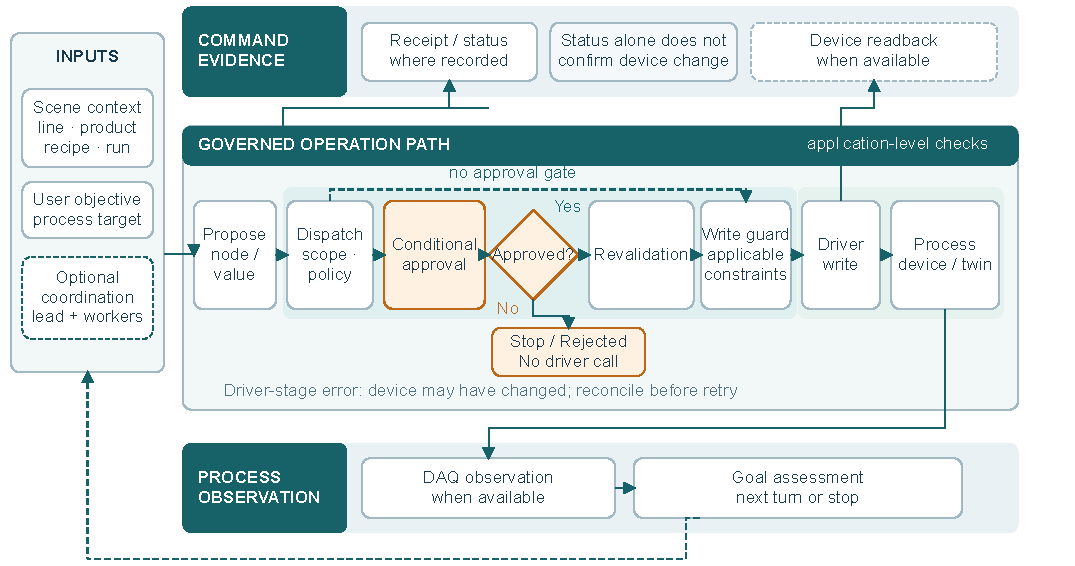
\includegraphics[width=0.98\textwidth]{resources/source/fig3/fig3-process-write-runtime.pdf}
\caption{Conceptual task-to-write flow. Approval is route-dependent: gated routes revalidate after approval; other routes bypass the gate and enter the shared write guard. A pre-dispatch rejection makes no driver call, whereas a driver-stage error may leave device state changed and requires reconciliation. Receipt, optional device readback, and later DAQ observation are distinct evidence. The figure describes the design, not an observed live-Agent success.}
\label{fig:agent-loop}
\end{figure*}
